\documentclass[letterpaper,12pt]{exam}
\usepackage[utf8x]{inputenc}
\usepackage{amsmath,anysize,graphicx,siunitx}
\usepackage[colorlinks]{hyperref}
\usepackage{python-commands}
\marginsize{1in}{1in}{1in}{0.5in}

\usepackage{epigraph}
\setlength\epigraphwidth{.7\textwidth}
\renewcommand{\epigraphflush}{center}
\setlength\epigraphrule{0pt}

\sisetup{per-mode=symbol}

\newcommand{\class}{CS 151}
\newcommand{\due}{Mon, Sept 18}

% Setting up headers and footers
\pagestyle{headandfoot}
\firstpageheader{PS2}{Intro to Python}{\class}
\firstpageheadrule
\firstpagefootrule
\firstpagefooter{Due \due}{}{\thepage}
\runningheadrule
\runningheader{}{}{\class}
\runningfooter{Due \due}{}{\thepage}
\runningfootrule

%\printanswers

\begin{document}
This problem set has one problem relating to Karel and then two problems concerning more generic Python programming. You should already be good to start working on the Karel problem, and the other problems you'll have most of the tools to solve after Wednesday. All problems have starting templates included in the repository. 
	\begin{center}
		Get Assignment link: \url{https://classroom.github.com/a/zZai6oXk}
	\end{center}
\begin{questions}
	%\begin{question}
		%The Python interpreter is particular about what sorts of variable names are allowed. For each of the listed names below, determine if that variable name would be considered legal by the interpreter. If it is not, state the reason why.
		%\begin{parts}
			%\part \pyi{your_name} \vspace{\stretch{1}}
			%\part \pyi[min]{friends4evar} \vspace{\stretch{1}}
			%\part \pyi{_if} \vspace{\stretch{1}}
			%\part \pyi{var} \vspace{\stretch{1}}
			%\part \pyi[min]{1var} \vspace{\stretch{1}}
			%\part \pyi{CATS} \vspace{\stretch{1}}
			%\part \pyi{my-name} \vspace{\stretch{1}}
			%\part \pyi[min]{and} \vspace{\stretch{1}}
		%\end{parts}
	%\end{question}

	%\newpage
	%\begin{question}
		%Do Exercise 4 from Chapter 1 in the book (pg 39). You should define the function such that it takes two arguments (x and y). The Github repository has a template to get you started. Make sure your function \emph{returns} the distance value in the end.
	%\end{question}
	%\vspace{\stretch{1}}

	%\begin{question}
		%Following up on its excellent painting skills, Karel has been hired to help usher in Spring! The trees are all bare from the winter, and need to have leaves added to their tops. Karel's goal then is to journey from tree to tree, adding a small square of leaves (in the form of beepers, naturally) at their tops. An example of the world before and after Karel does its work is below:
		%\begin{center}
			%\begin{tikzpicture}[scale=0.7, transform shape]
				%\karelgrid{14}{6}
				%\karelmark{1}{1}{0}
				%\draw[very thick] (2.5,0.5) --+(0,2)
								  %(4.5,0.5) --+(0,4)
								  %(8.5,0.5) --+(0,4)
								  %(11.5,0.5) --+(0,3);
				%\node at (7,7) {Before};
			%\end{tikzpicture}

			%\newcommand{\leaves}[2]{
				%\karelbeeper{#1}{#2}
				%\karelbeeper{#1+1}{#2}
				%\karelbeeper{#1}{#2+1}
				%\karelbeeper{#1+1}{#2+1}
			%}
			%\begin{tikzpicture}[scale=0.7, transform shape]
				%\karelgrid{14}{6}
				%\karelmark{14}{1}{0}
				%\draw[very thick] (2.5,0.5) --+(0,2)
								  %(4.5,0.5) --+(0,4)
								  %(8.5,0.5) --+(0,4)
								  %(11.5,0.5) --+(0,3);
				%\leaves{2}{3}
				%\leaves{4}{5}
				%\leaves{8}{5}
				%\leaves{11}{4}
				%\node at (7,7) {After};
			%\end{tikzpicture}
		%\end{center}

		%This is an excellent problem to practice step-wise refinement and breaking the overall problem into smaller, more manageable pieces. You are guaranteed that:
		%\begin{itemize}
			%\item Karel starts in the bottom left corner facing to the east.
			%\item Karel has just enough beepers in its bag to add foliage to all the trees in the world.
			%\item No trees are so tall that their leaves would extend off the top of the world.
			%\item No tree's leaves will overlap with another tree's leaves.
		%\end{itemize}
		%What you are \emph{not} guaranteed is the number of trees and where they are placed within the world. In addition, once Karel has added leaves to the last tree, it is to finish the program in the bottom right corner, facing east. Several alternative ``forests'' in addition to the above example have been included in the repository for you to test your code against (\texttt{Forest1.w} and \texttt{Forest2.w}). For full points your program should successfully add leaves and end in the correct position for the default world and both forests as well showing evidence of how you have used decomposition and functions to break the problem into smaller pieces. Comments should be used to explain what each function does/is responsible for.
		
	%\end{question}

	\begin{question}
		Karel, tired of painting, is thinking more abstractly, and wants to lay out a checkerboard pattern of beepers inside an empty rectangular world. An example of a before and after for an 8x8 world is shown below:
		\begin{center}
			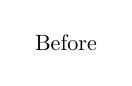
\begin{tikzpicture}[scale=.8, transform shape]
				\karelgrid{8}{8}
				\karelmark[fill=white]{1}{1}{0}
				\node at (4.5,-1) {Before};
			\end{tikzpicture}
			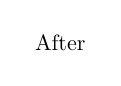
\begin{tikzpicture}[scale=.8, transform shape]
				\karelgrid{8}{8}
				\karelmark[fill=white]{1}{8}{90}
				\node at (4.5,-1) {After};
				\foreach \x in {1,3,5,7} {
					\foreach \y in {1,3,5,7} {
						\karelbeeper[fill=gray!50]{\x}{\y}
					}
				}
				\foreach \x in {2,4,6,8} {
					\foreach \y in {2,4,6,8} {
						\karelbeeper[fill=gray!50]{\x}{\y}
					}
				}
			\end{tikzpicture}
		\end{center}

		This problem has a nice decomposition structure along with some interesting algorithmic issues. As you think about how you will solve the problem, you should make sure that your solution works with checkerboards that are different in size from the standard 8x8 checkerboard shown in the example above. Odd-sized checkerboards are trickier, and you should make sure that your program generates the following pattern in a 5x3 world:
		\begin{center}
			\begin{tikzpicture}[scale=0.8]
				\karelgrid{5}{3}
				\foreach \x in {1,3,5}{
					\foreach \y in {1,3}{
						\karelbeeper[fill=gray!50]{\x}{\y}
					}
				}
				\foreach \x in {2,4} \karelbeeper[fill=gray!50]{\x}{2};
				\karelmark[fill=white]{5}{3}{90}
			\end{tikzpicture}
		\end{center}

		Another special case you need to consider is that of a world which is only one column wide or one row high. The repository includes several sample worlds for you to test your program against, including: \texttt{1x8.w}, \texttt{5x3.w}, \texttt{5x5.w}, and \texttt{8x1.w}. You can safely assume that Karel always starts in the bottom left corner and facing to the east with an infinite supply of beepers in its bag. In does not matter where Karel finishes (but they should finish without erroring!) or which specific spaces have beepers, except that the world should be completely checkerboarded. To get full points on this problem, your program should show clear evidence of how you decomposed the problem and successfully recreate a checkerboard on any empty rectangular world.
	\end{question}

	%\begin{question} Taken from Chapter 1, exercise 7.
		%%Do Exercise 6 from Chapter 1 in the book (pg 40). I've already provided you with the template file \texttt{Prob3.py}. Add your three functions there. Make sure that each function is returning the desired string, not just printing it! I've also included the example console session from the book in the \pyi{if __name__ == '__main__':} portion of the code so you can just run the code to see if the correct terms are printed.

		%\epigraph{\itshape It is a beautiful thing, the destruction of words.}{---Syme in George Orwell's \textit{1984}}

		%In Orwell's novel 1984, Syme and his colleagues at the Ministry of Truth are engaged in simplifying English into a more regular language called \emph{Newspeak}. As Orwell describes in his appendix entitled ``The Principles of Newspeak,'' words can take a variety of prefixes to eliminate the need for the massive number of words we have in English. For example, Orwell writes,

%\renewcommand{\textflush}{flushepinormal}
		%\epigraph{Any word---this again applied in principle to every word in the language---could be negatived by adding the affix \emph{un-}, or could be strengthened by the affix \emph{plus-}, or, for still greater emphasis, \emph{doubleplus-}. Thus, for example, \emph{uncold} meant ``warm'', while \emph{pluscold} and \emph{doublepluscold} meant, respectively, ``very cold'' and ``superlatively cold.''}

		%Define three functions---\pyi{negate}, \pyi{intensify}, and \pyi{reinforce}---that take a string as input and add the prefixes \pyi{"un"}, \pyi{"plus"}, or \pyi{"double"} to that string, respectively, returning the result. For instance, if you were to enter in \pyi{negate("cold")} you should get out the string \pyi{"uncold"}. Below are several more examples of expected input and output, including chaining these functions together. These are all also printed in the given template so that you can check your code.
		%\begin{center}
			%\begin{tabular}{rl}
				%\pyi{negate("cold")} $\rightarrow$ & \pyi{"uncold"} \\
				%\pyi{intensify("cold")} $\rightarrow$ & \pyi{"pluscold"} \\
				%\pyi{reinforce(intensify("cold"))} $\rightarrow$ & \pyi{"doublepluscold"} \\
				%\pyi{reinforce(intensify(negate("good")))} $\rightarrow$ & \pyi{"doubleplusungood"}\\
			%\end{tabular}
		%\end{center}


	%\end{question}

	\begin{question}
	I'm supplying you with a template file for this problem, but it is largely empty. You thus have lots of flexibility in how you want to approach this, but make sure it achieves the objectives.

		\epigraph{\itshape Why is everything either at sixes or at sevens?}{---Gilbert and Sullivan, \emph{H.M.S. Pinafore}, 1878}

		Write a function called \pyi{divisible_by_six_or_seven} which takes two arguments as input. The first argument should represent the lower bound of a series of numbers to check, whereas the second argument should represent the upper bound. So for instance, calling \pyi{divisible_by_six_or_seven(1,100)} should check the numbers from 1 to 100 (including 1 and 100). Your function should print a number to the screen from the provided range if and only if it is evenly divisible by six or seven, \emph{but not both}. These numbers do \textbf{not} need to be in strictly ascending order. In addition to printing these numbers, your function should keep track of how many numbers are printed, and \emph{return} this value at the end of the function. So for instance, one example of running the program in the Python REPL might look like:
		\begin{pythoncode}[style=min]
			>>> count = divisible_by_six_or_seven(40, 60)
			49
			56
			48
			54
			60
			>>> print(count)
			5
		\end{pythoncode}
	\end{question}

	\newpage
	\begin{question}
		Consider the situation in which you have two perfect squares, one with a side length of $A$ and the other with a side length of $B$, positioned as shown below. 
		\begin{center}
			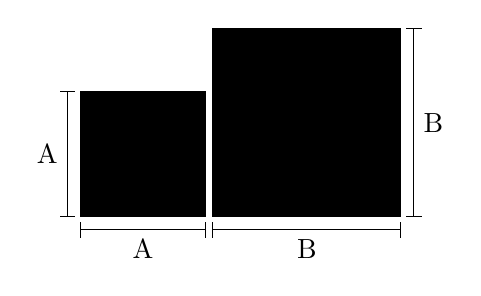
\begin{tikzpicture}[scale=.8]
				\fill[black] (0,0) rectangle + (3,3);
				\fill[black] (-.1,0) rectangle +(-2,2);

				\draw[|-|] (0,-.2) -- +(3,0) node[midway,below] {B};
				\draw[|-|] (-.10,-.2) -- +(-2,0) node[midway,below] {A};
				\draw[|-|] (3.2,0) -- +(0,3) node[midway,right] {B};
				\draw[|-|] (-2.3,0) -- +(0,2) node[midway,left] {A};
			\end{tikzpicture}
		\end{center}

		Initially, there is no overlap and the total shaded area encompassed by both squares would be equal to $A^2 + B^2$.

		Now suppose that the squares are moved towards one another such that they overlap a distance $d$, where $d$ is 0 at a minimum and $A$ at a maximum. (\emph{See animated gif in the HW Images folder if you are having trouble picturing this over the full range.}) The total shaded area has clearly gone down.
		\begin{center}
			\def\d{-1}
			\begin{tikzpicture}[scale=.8]
				\fill[black, opacity=0.9] (\d,0) rectangle + (3,3);
				\fill[black, opacity=0.9] (-.1,0) rectangle +(-2,2);
				\draw[|-|] (0,3.3) -- +(\d,0) node[midway,above] {d};
			\end{tikzpicture}
		\end{center}

		Your objective in this problem is not to actually write a Python script, but to instead write out in plain English what your algorithm would be for computing the total area covered by the squares for any given values of $A$, $B$, and $d$, where you are promised that $A > 0$, $B > 0$ and $0 \leq d \leq A$.

		In the provided template, write out using words and full sentences what your approach would be to find the total shaded area. No coding needs to be happening here, you just need to determine a method by which you can find the total covered area and convey that method clearly in English. Imagine that someone with no knowledge of this specific problem should be able to implement your described algorithm just from your description, and have it work for all possible values of $A$, $B$, and $d$.
			
			\emph{Reminders and Tips:
			\begin{itemize}
				\item You just need the shaded area, so be careful you don't ``double count'' the overlapping region.
				\item You don't know which square is larger, so you may need your algorithm to adjust depending on the inputs.
				%\item Breaking the area up into smaller pieces may be helpful.
				\item It might be useful to map out the major possible configurations to ensure your algorithm works for all of them.
			\end{itemize}
			}

				

	\end{question}
	
\end{questions}


\end{document}
